%% NOTES:
%%    do we want to explore for larger S?  Does false positive rate change?

% review: first round, chris, enbody, cole/jordan?
% second round yanni, curt, james foster

\documentclass[12pt]{article} \usepackage{simplemargins}
\usepackage[pdftex]{graphicx} \graphicspath{{figures/}}

\setlength{\parindent}{0pt} \setlength{\parskip}{1.6ex}
\setallmargins{1in} \linespread{1.6}

\begin{document}

\title{A probabilistic framework for compressible assembly graphs}
\author{Jason Pell, Arend Hintze, Rosangela Canino-Koning, C. Titus Brown}

\maketitle

\section{Abstract}

We introduce a fast and lightweight representation for DNA k-mer graphs
based on Bloom filters, a constant-memory probabilistic data structure that allows us
to compress graphs.  This graph has a one-sided
error that is precisely tunable and yields predictable degradation of
graph properties as memory usage is decreased. We show that degradation of global graph connectivity with an increasing false
positive rate relates to percolation theory. Through 
simulation, we find that percolation for random graphs occurs at a false positive rate 
of $\sim 0.183$, independent of k. We discuss ways that this
graph representation can be used to scale de novo DNA sequence assembly by characterizing the structure of
large assembly graphs.

\section{Introduction}

Within the past decade, the volume of sequence data generated
from next-generation sequencing platforms such as Illumina and 454
has outpaced the computational resources needed for
analysis. Currently, the memory needs for sequencing projects 
are high. Recent metagenomic sequencing efforts such as the human gut
microbiome\cite{pmid20203603}, cow rumen\cite{pmid21273488}
require large computers with 512GB of memory
or more to construct their assemblies.  This is also true of resequencing
efforts for e.g the human genome\cite{pmid21187386}.
\marginpar{Reference the BGI resequencing/assembly paper, too.}
Sequencing companies continue to innovate in developing new 
methods to produce longer reads
and deeper coverage. However, this further contributes 
to the difficulty in scaling computational 
analysis of the data, and better approaches are needed.
Today, high memory requirements are
among the biggest bottlenecks that we face in sequence assembly.

The goal of de novo assembly is to combine individual disconnected
reads into a consensus sequence based on overlaps and mate-pair
information.
%% Before the advent of next-gen platforms, Sanger
%%sequencing was the primary method used for sequencing. To assemble 
%%this type of data, the reads are checked for overlaps through an 
%% all-by-all comparison, and an overlap graph is created\cite{assemblyreview}.
%% Using the overlap graph, the assembler 
%% performs multiple sequence alignments to find a consensus sequence. 
%% If paired-end information is available, repetitive regions in the 
%% genome are resolved, and scaffolds between contigous sequences are 
%% created. This class of assemblers is generally called 
%% ``Overlap-Layout-Consensus.'' Examples include
%%Arachne\cite{arachne}, Celera\cite{celera}, Newbler\cite{newbler}, and 
%%PCAP\cite{pcap}. However, with next-gen sequencing 
%%platforms such as 454 and Illumina, much larger datasets of shorter reads 
%%are generated. With the Illumina Hi-Seq 2000 platform, up to 200 
%%gigabases of sequence can be generated 
%%in around 7 days. The assembly of 
%%these reads requires different
%%algorithms due to their shorter read length but also a 
%%large amount of memory.
Originally developed to 
handle repeat structures in Sanger datasets, a new approach using de Bruijn 
graphs (DBG) was developed\cite{pmid11504945}, which scales in terms of 
memory with the amount of novel sequence as opposed to reads.
In a de Bruijn
graph approach, reads are broken down along a sliding window into words of fixed
size $k$, or k-mers, and overlaps are represented within the graph 
structure.
De Bruijn graph assemblers then try to build an Euler path through
this graph, which are outputted as assembled contigs\cite{assemblyreview}.
\marginpar{Reference meraculous, too.}

As next-generation sequencing platforms became prominent, the DBG approach
became the preferred method for assembling these types of datasets
because an all-by-all comparison of reads is infeasible in situations where 
computational resources are limited relative to the size of the data 
sets.  However, it
is clear that new methods are needed to handle the
increasing size of sequence datasets. This need is
particularly prevalent in the area of metagenomics and mRNAseq.  Both
metagenomics and mRNAseq require deep sampling to detect rare species;
this deep sequencing introduces many new k-mers through error.

Driven by the need to scale assembly, we explore the novel use of a 
Bloom filter variant data structure to create a compressible graph 
representation. Bloom filters\cite{bloom} have been used for 
Bioinformatics applications 
in the past\cite{pmid20472541, haskell, pmid20426693} but not for graph 
storage.
\marginpar{More summary needed here.}
We show that our method drastically
reduces memory requirements for graph storage and analysis, and that the effects
of the false positive rate are negligible, especially relative to the errors
introduced by modern sequencing platforms.
We also demonstrate that our 
approach performs well below a specific false positive rate. Finally, we 
briefly discuss techniques for using the probabilistic k-mer graph 
to study assembly graph structure and potentially improve assembly by 
graph decomposition, repeat filtering, and other approaches.

\section{Methods}

\subsection{Data Structure Implementation}
\marginpar{OK, this needs to be elaborated!  We store... we retrieve... perhaps a little intro to Bloom filters...}
% @JAP I added and merged some stuff, but I think the language needs to be 
% more ``direct''
We implemented a variation of the Bloom filter data structure to store k-mers
in memory. In a classic Bloom filter, multiple hash functions map into 
a single hash table to add an object or test for the presence of an object 
in the set. In 
our variant, we use multiple hash tables with different hash functions. 
To add a k-mer to the filter, the corresponding bit is set to 1 
if it is not already set.  
To find the presence of a k-mer, each table is queried for the
presence of a k-mer until the k-mer cannot be found in a hash
table. In order for a k-mer to be considered present in the dataset, 
the k-mer must be found in all of the hash tables. On the other hand, 
if a k-mer is not present in even one hash table, then it is certainly 
not in the dataset. As a result, there is a one-sided error where 
false positives are possible but false negatives are not. As with other 
hash-style data structures, Bloom filters have a
fast lookup time, which is $O(h)$ when there are $h$ hash tables to query
for k-mer presence.

\subsection{Using The Bloom Filter As A K-mer Graph}
\marginpar{Should we use node and vertex interchangeably, or settle on one?}
Having stored the k-mers into a Bloom filter, we are able to traverse
the data as a k-mer graph. We let each k-mer be a vertex, where
the reverse complement of a k-mer is considered the same
vertex. Each k-mer can
have up to eight neighbors, which are any of the other k-mers that
 share a $k-1$
overlap; no explicit edge is created. In doing so, we implicitly 
treat the graph as a simple graph as opposed to a multigraph or 
digraph, which means that there can be no self-loops or parallel 
edges between vertices/k-mers. Our graph representation is constant 
in its memory usage, so only ancillary information such as list 
of vertices visited or waypoints in the graph consume addition 
memory.\marginpar{This last point seems a bit abrupt.  Should we expand?}
In contrast to an exact approach, there is a chance that a k-mer 
will be adjacent to a false positive,
that is, a k-mer
that does not actually exist in the original dataset due to the false
positive rate from the Bloom filter. If this probability is too high, the 
graph can become unusable since the false k-mers dominate the graph 
and erroneously connect components.
Intuitively, it is clear that when most real k-mers
have at least one erroneous neighbor ($p_f \approx \frac{1}{8}$), 
false paths between real (but unconnected) k-mers are likely to 
appear. However, it is not immediately clear at exactly what 
false positive rate this occurs in the absence of an analytic
solution.  We address this below.  % clumsy, I know.
\marginpar{Do we discuss end-to-end false positives anywhere?  We should.}
Note that this graph structure is effectively compressible 
because one can choose a larger
or smaller size for the underlying Bloom filters; a larger size admits fewer
false positives, while a smaller size admits more. By relying on Bloom
filters, the data structure is effectively constant memory: no extra memory is
used as additional data is added. However, as memory is decreased or data
is increased, only false positive vertices and edges are gained, so
compressing the graph results in a more tightly interconnected graph.
\marginpar{Do we want to put in the ``paper crumpling'' analogy?}

\subsection{Calculating Data Structure Properties}
The properties of our Bloom filter variant, which 
uses a separate hash table for each hash function, are essentially the 
same as a classical Bloom filter. To calculate the false positive rate, we 
take the product of the occupancy of each hash table; that is,
\begin{displaymath}
P_f = \prod_{h \in H} occ(h)
\end{displaymath}
where $h$ is a hash table in the set of hash tables $H$, $occ$ denotes 
the occupancy (proportion of bits set) for a hash table.
We find the optimal number of hash tables 
to use by calculating
\begin{displaymath}
\vert H \vert_{opt} = \ln 2 \frac{m}{k}
\end{displaymath}
where $m$ is the amount of memory in bits to allocate and $k$ 
is the number of k-mers to be inserted (@CTB reference?). Finally, 
the number of bits per 
k-mer used in the data structure is 
\begin{displaymath}
\frac{m}{n} = \frac{1}{\ln(2)} \log{\frac{1}{P_f}}.
\end{displaymath}
% @JAP re: references for this section
% this math is pretty straightforward to derive, but I have found a 
% paper called Summary Cache: A Scalable Wide-Area Web Cache 
% Sharing Protocol that does the relevant math if we want to use it

\subsection{Estimating False Positive Rate Of Erroneous Connectivity}
We ran a simulation to find when connected components in the graph 
begin to erroneously connect to one another.
To calculate the false positive rate at which this aberrant 
connectivity occurs, 
we added random k-mers to the data structure 
and then calculated the false positive rate and size of 
the largest connected 
component. This allowed us to sample the relative size of 
the largest component for every 
given $p$ (probability that any given (@CTB?) k-mer is present) as well as the cluster size distribution. 
At the percolation threshold this cluster size distribution must be scale-free (citation?). \marginpar{Is this true for finite graphs?}
We then found at what value of $p$ the resulting 
distribution in logarithmic 
scale can be better fitted in a linear or quadratic fashion using 
the F-value (reference?)
\newline
\newline
\begin{displaymath}
F=\frac{\frac{RSS_1-RSS_2}{p_2-p_1}}{\frac{RSS_2}{n-p_2}}.
\end{displaymath}
Finally, to handle the finite size sampling error, the data was binned using the 
threshold binning method\cite{adami2002critical}. The critical value for 
when aberrant connectivity occurred was found by finding the local maxima.

\subsection{Software and Software Availability}
We have implemented this compressible graph representation in a software package
named khmer.
It is written in C++
and Python 2.6 and is available under the BSD open source license at
https://github.com/ctb/khmer.
The graphviz software 
package was used for graph visualizations. The scripts to 
generate the figures of this paper are available in the khmer repository.

\section{Results}

\subsection{Effect Of False Positives on Local Graph Structure}
We wanted to see understand how erroneous neighbors created 
by false positives can alter 
the local graph structure, so we randomly generated a 1,031bp circular sequence .
Then, storing this sequence in compressible graphs with
four different false positive rates ($p_f$=0.01, 0.05, 0.10, and
0.15), we explored the graph using breadth-first search beginning at
the first 31-mer. 
The graphs in Figure 
1 demonstrate how
the local graph structure begins to elaborate while the original circular
graph remains intact with no erroneous paths between k-mers that are
truly present in the originally generated sequence. Because the k-mer
space is extremely large for large k, a relatively high false positive 
rate ($\sim$ 15\%) is still 
unlikely to connect components
together erroneously. We also note that when the false positive
rate is sufficiently high, the resulting graph would be
(practically speaking) impossible to visualize for high values of $k$ (e.g. $\ge 25$). 
\marginpar{I thought the argument of fp=15 being ok has nothing to do with
the size of the k-mer space?  Or is this a separate argument?}
% @JAP what I tried to say was that you can easily visualize when k=4, 5, 6, 
% for _any_ false positive rate, but at k=30, you can't

\begin{figure}
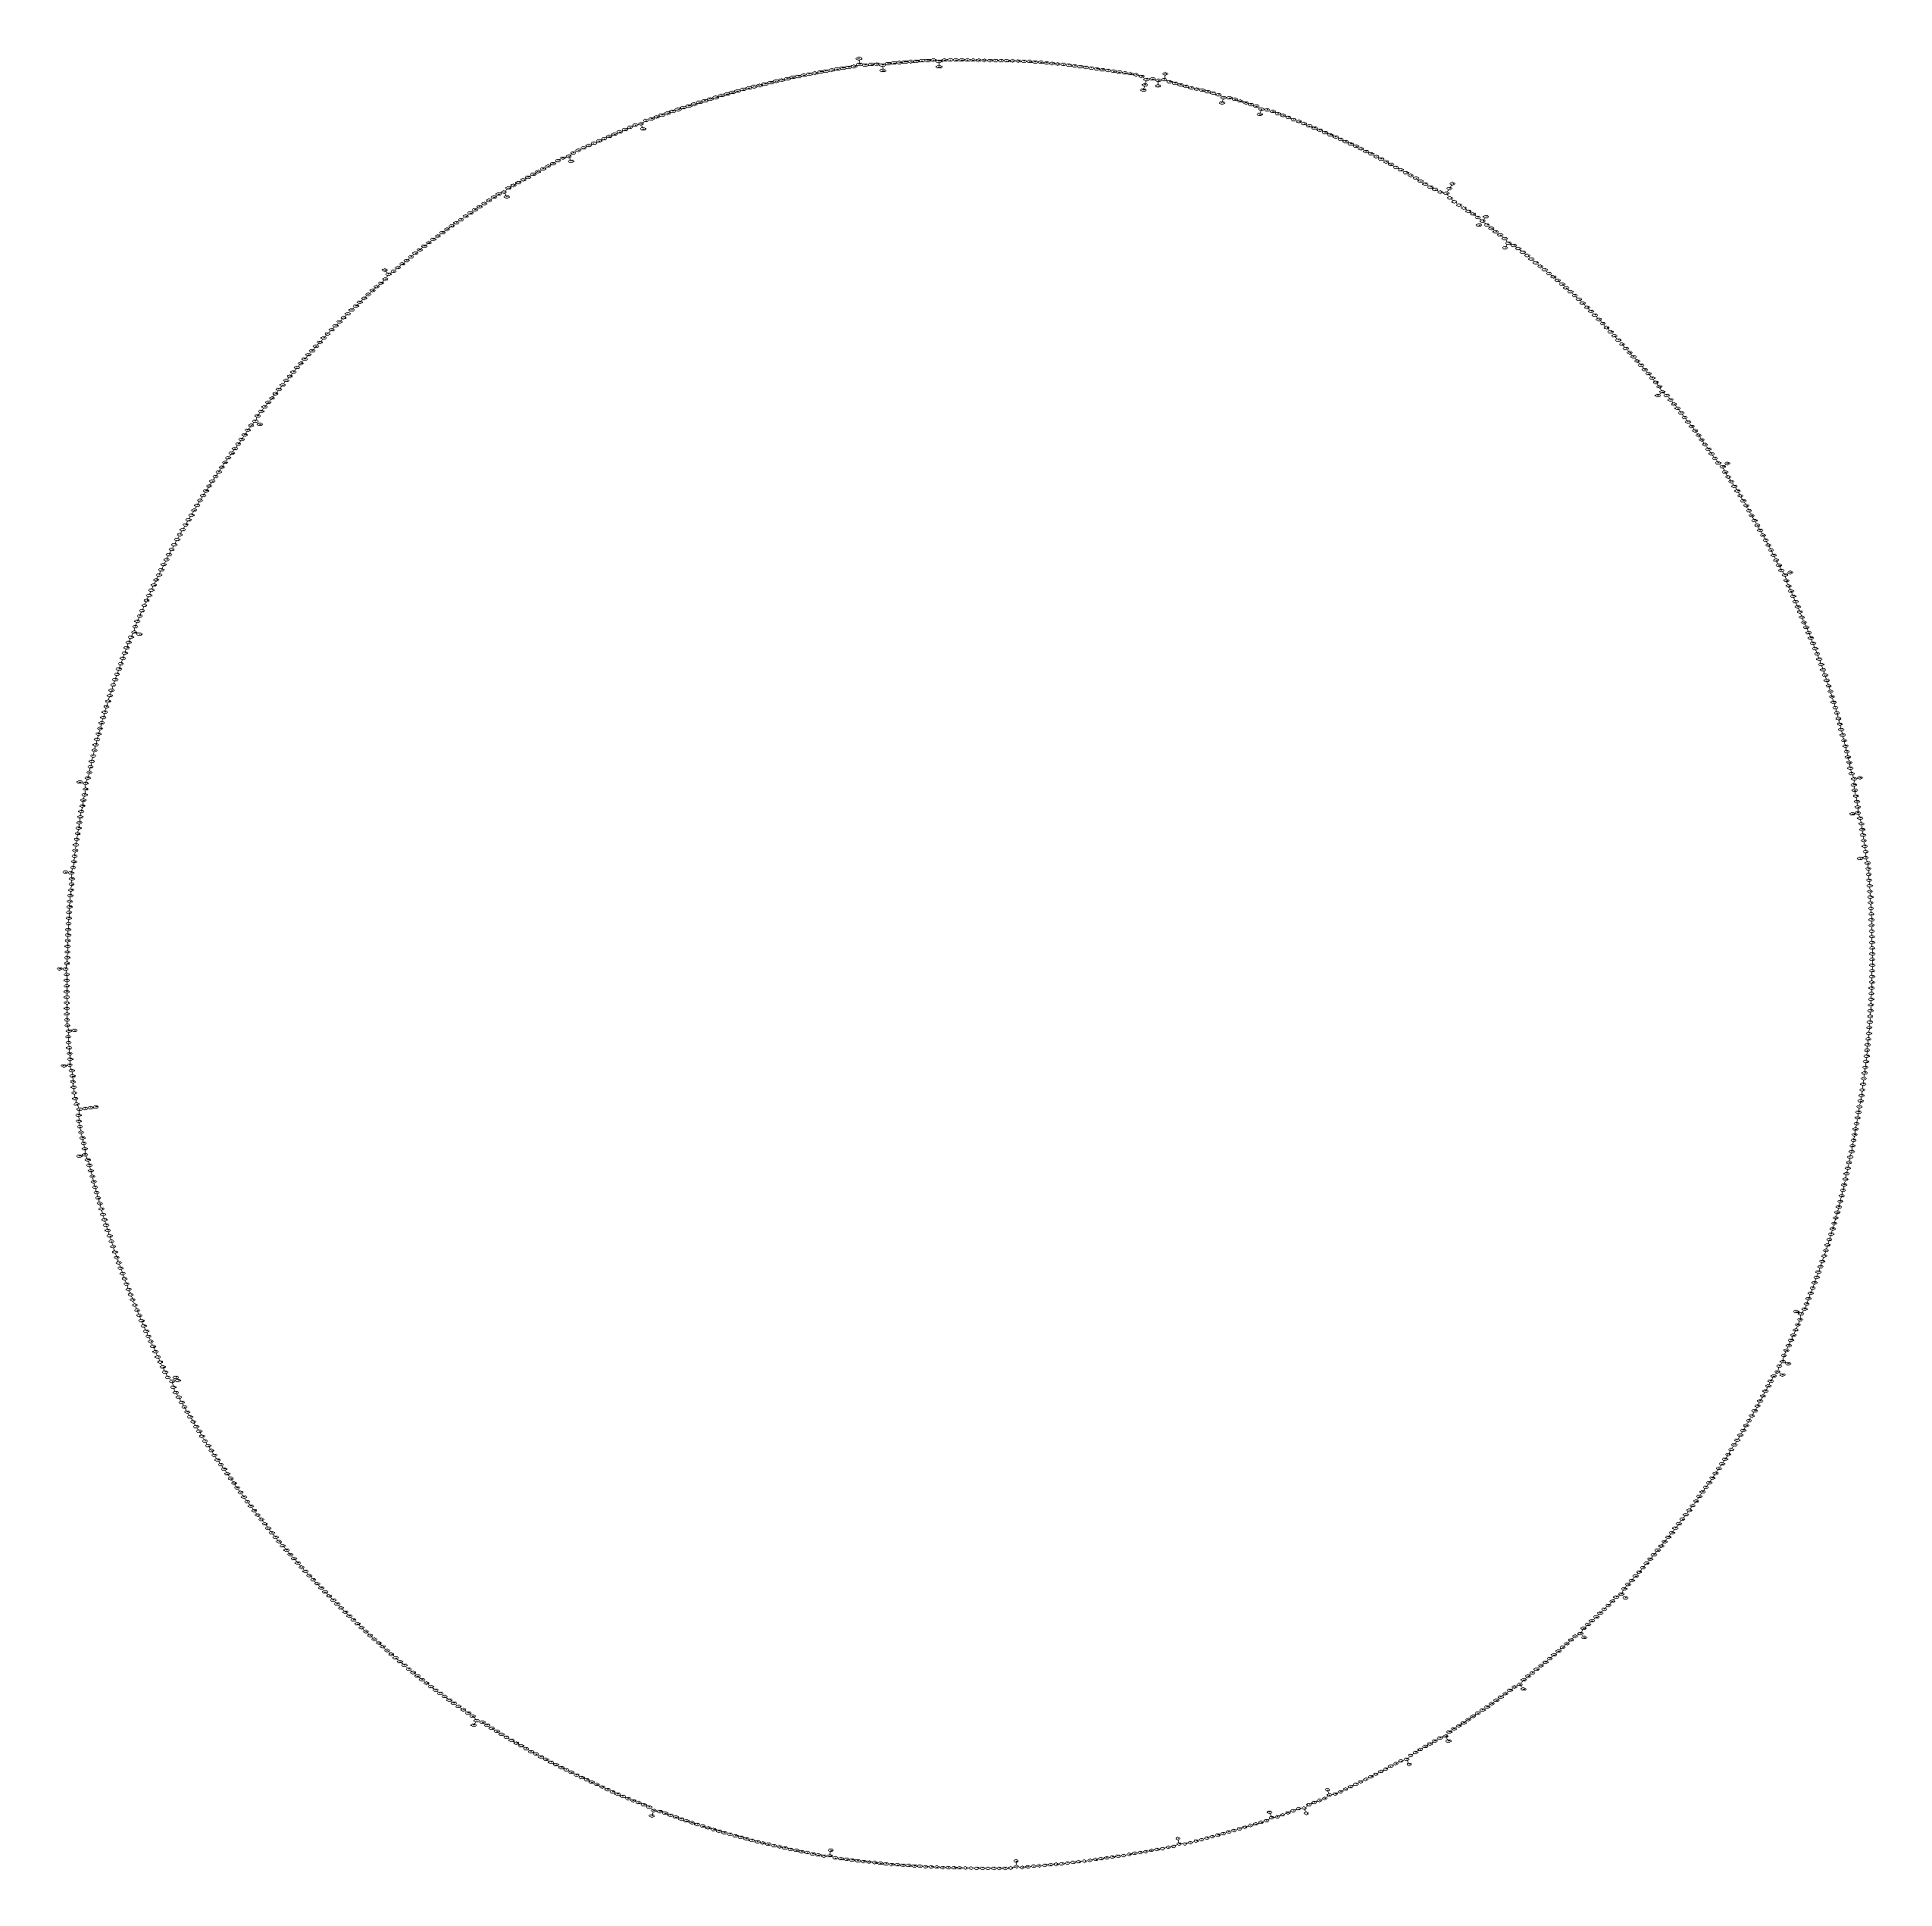
\includegraphics[width=3in]{figures/f3b001}
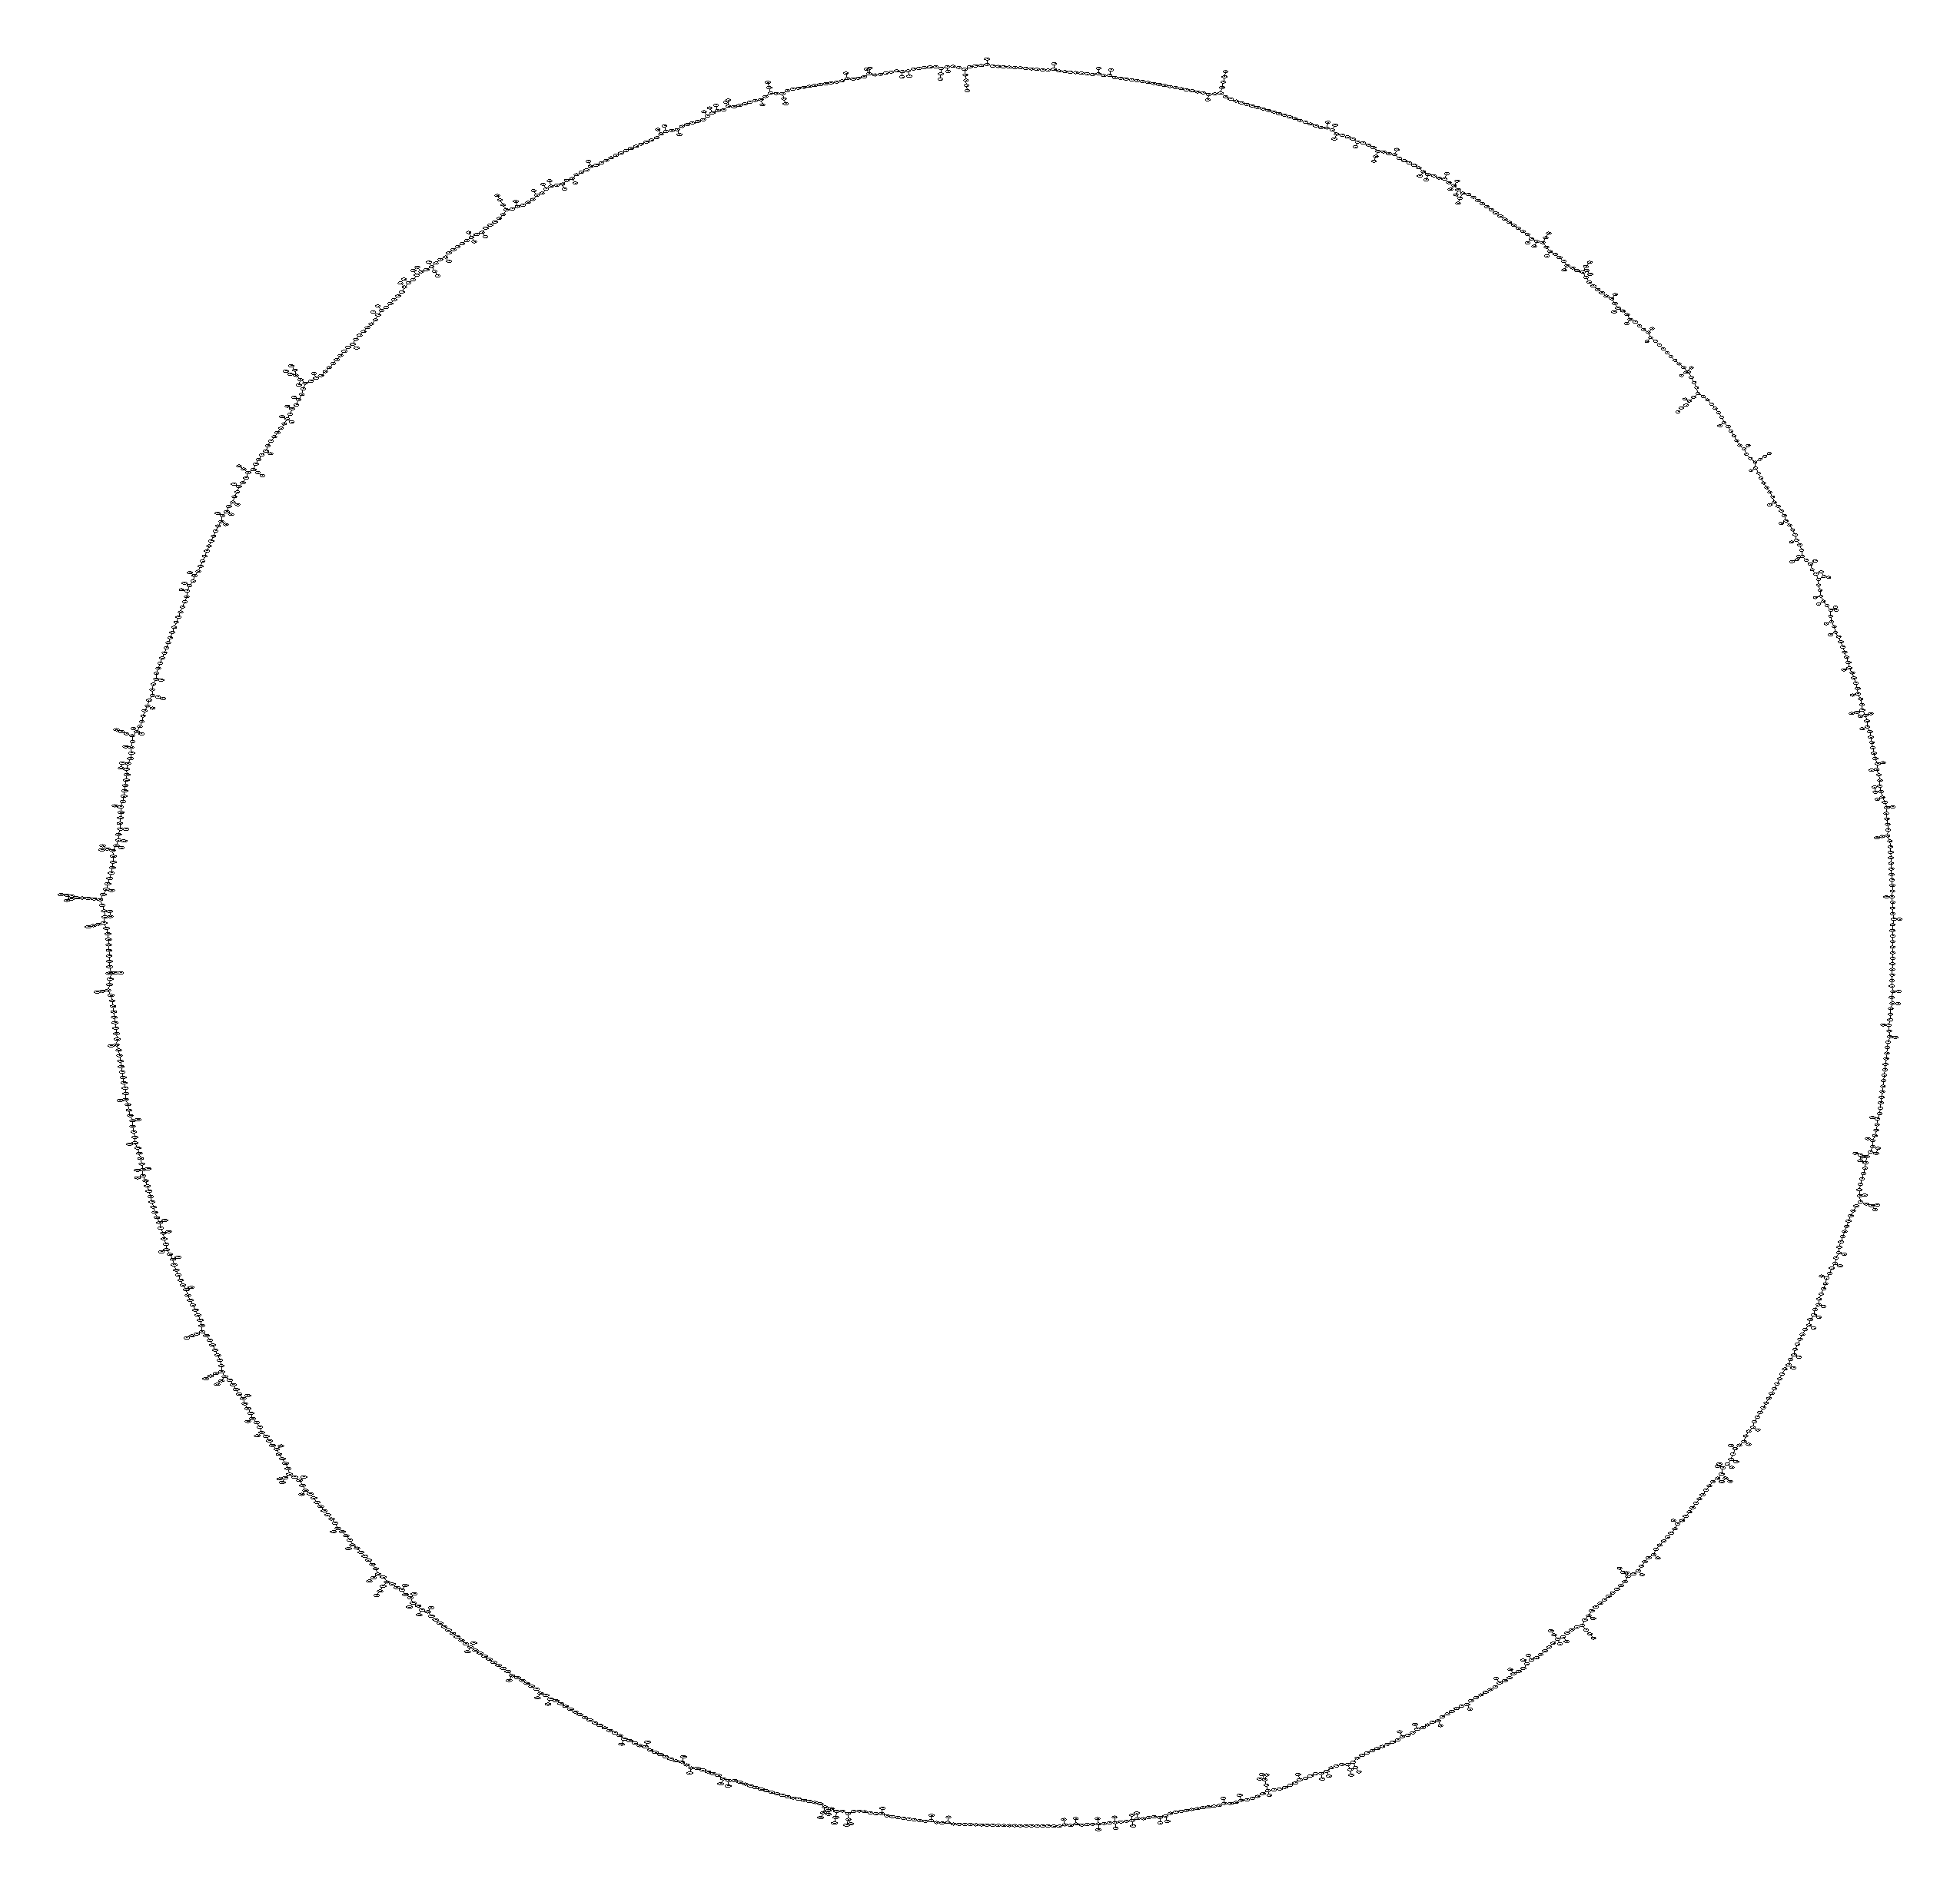
\includegraphics[width=3in]{figures/f3b005}\\
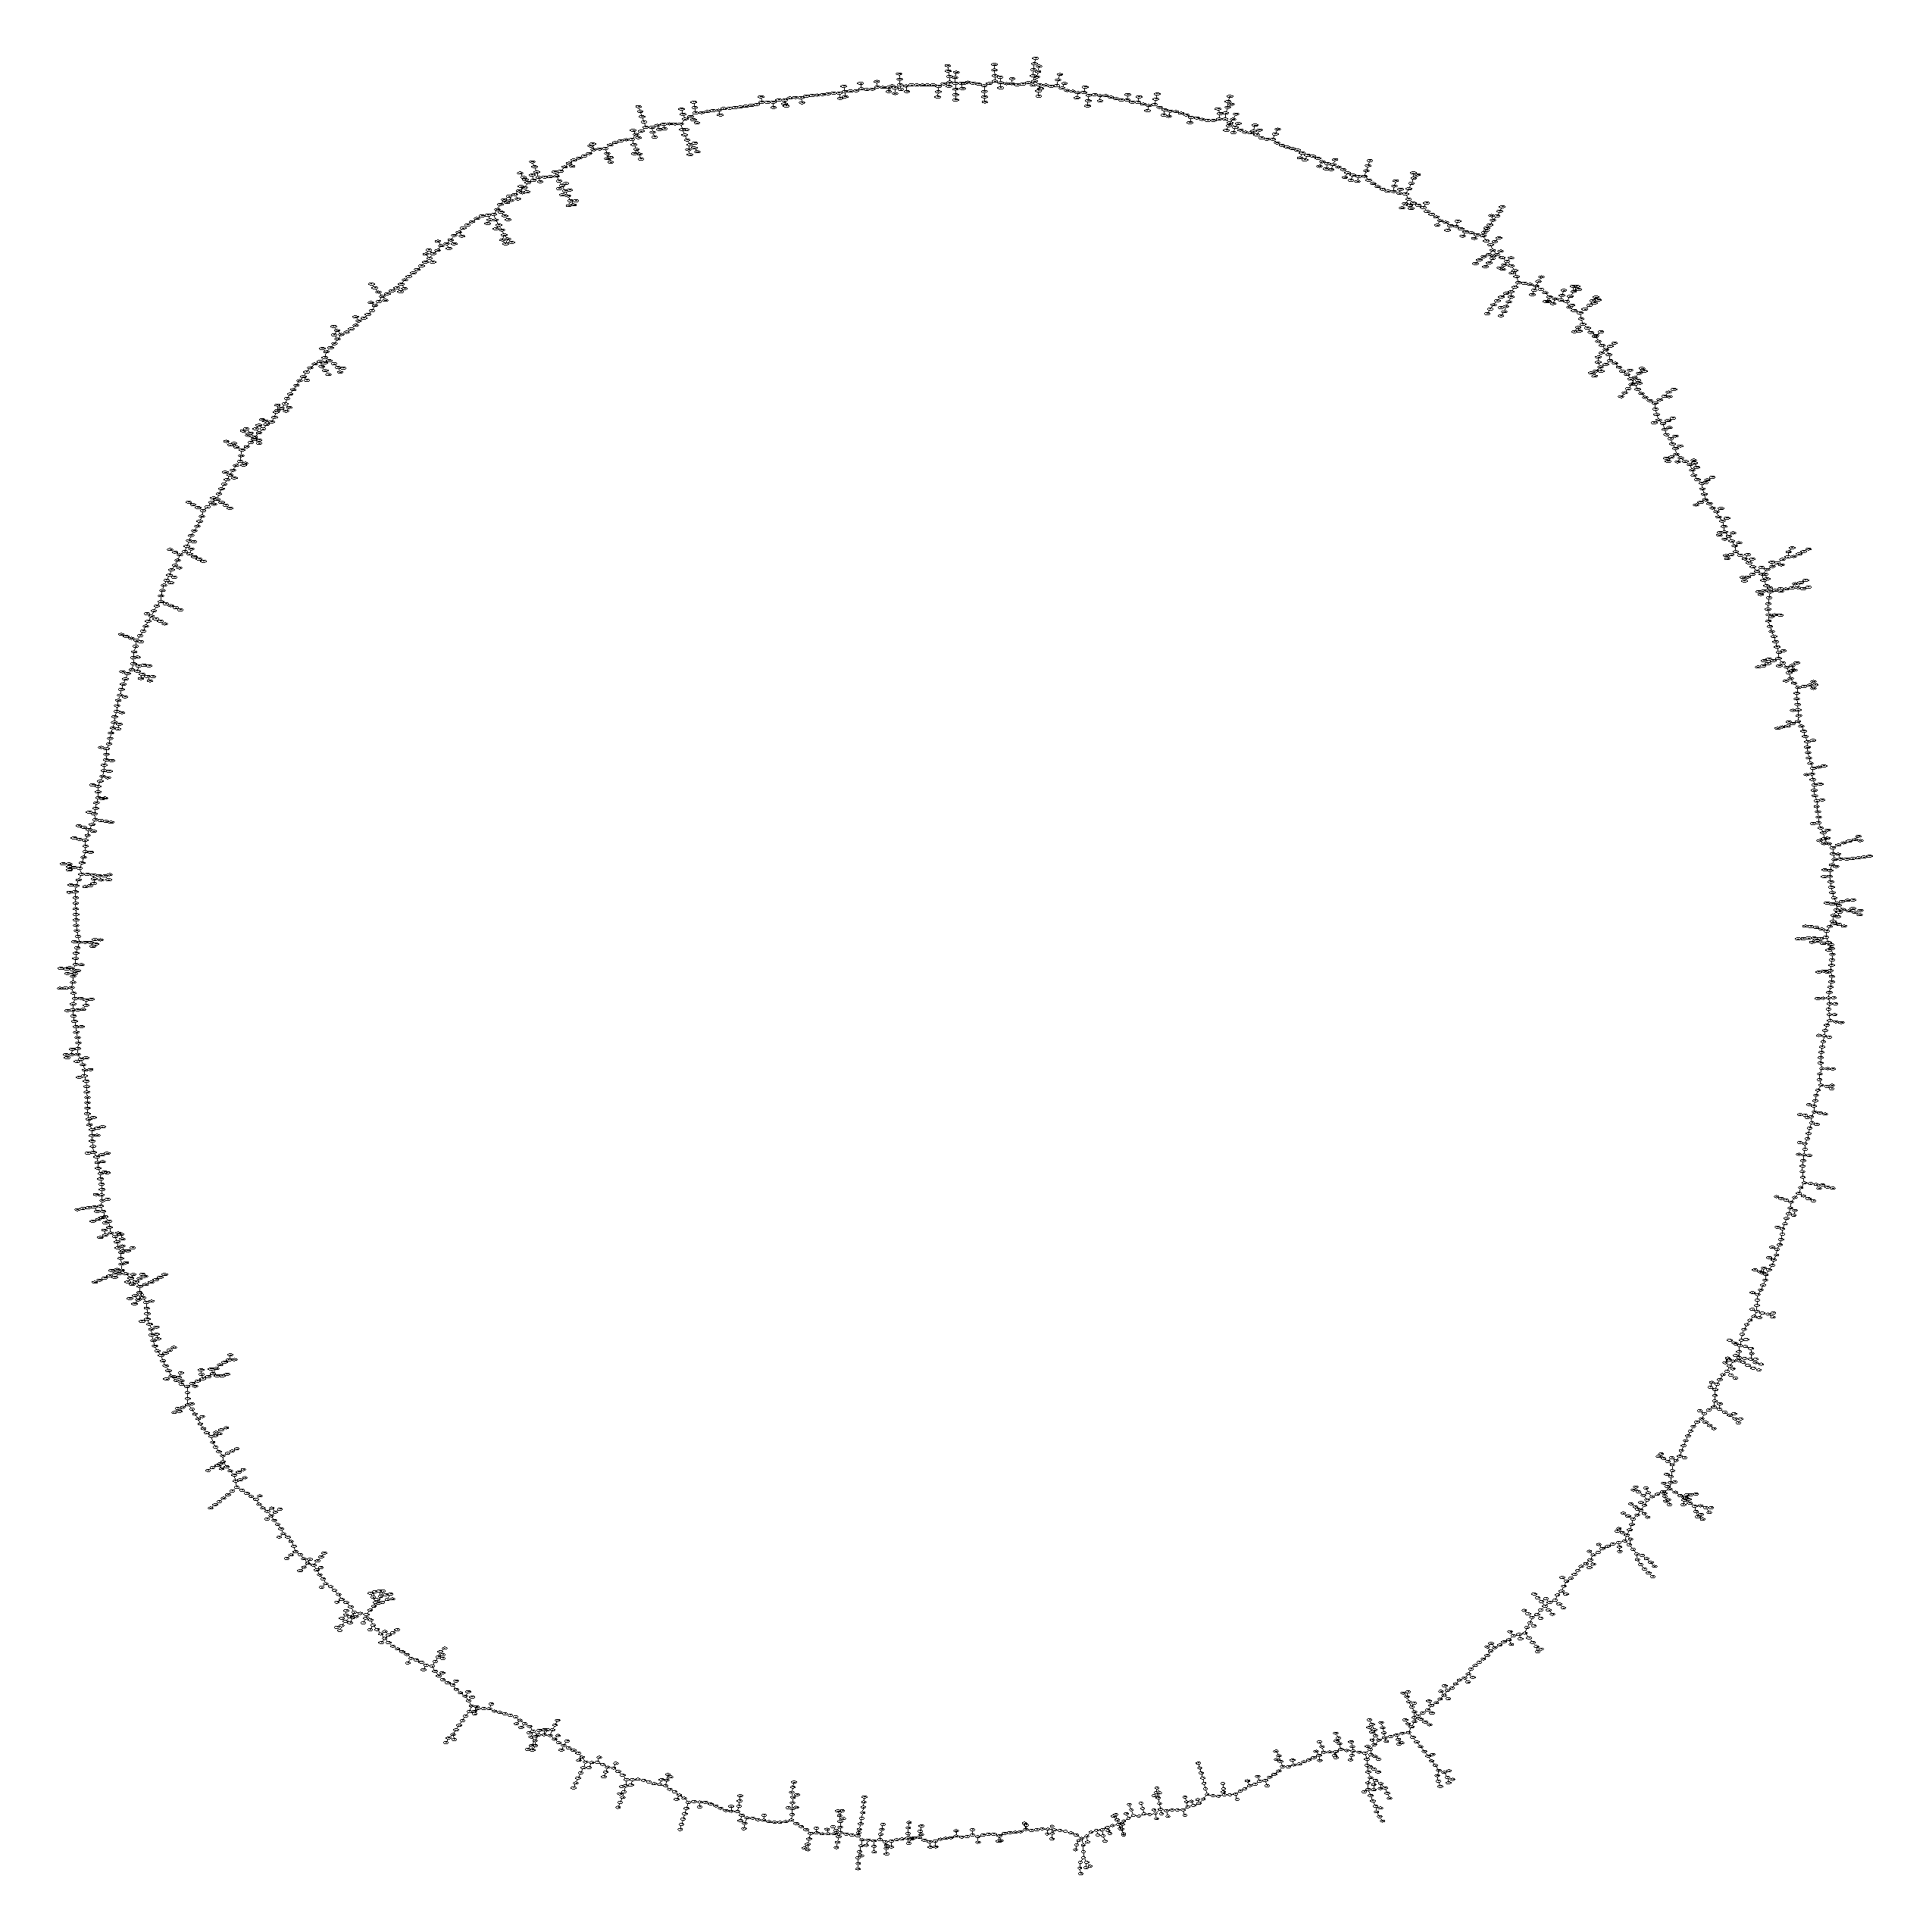
\includegraphics[width=3in]{figures/f3b010}
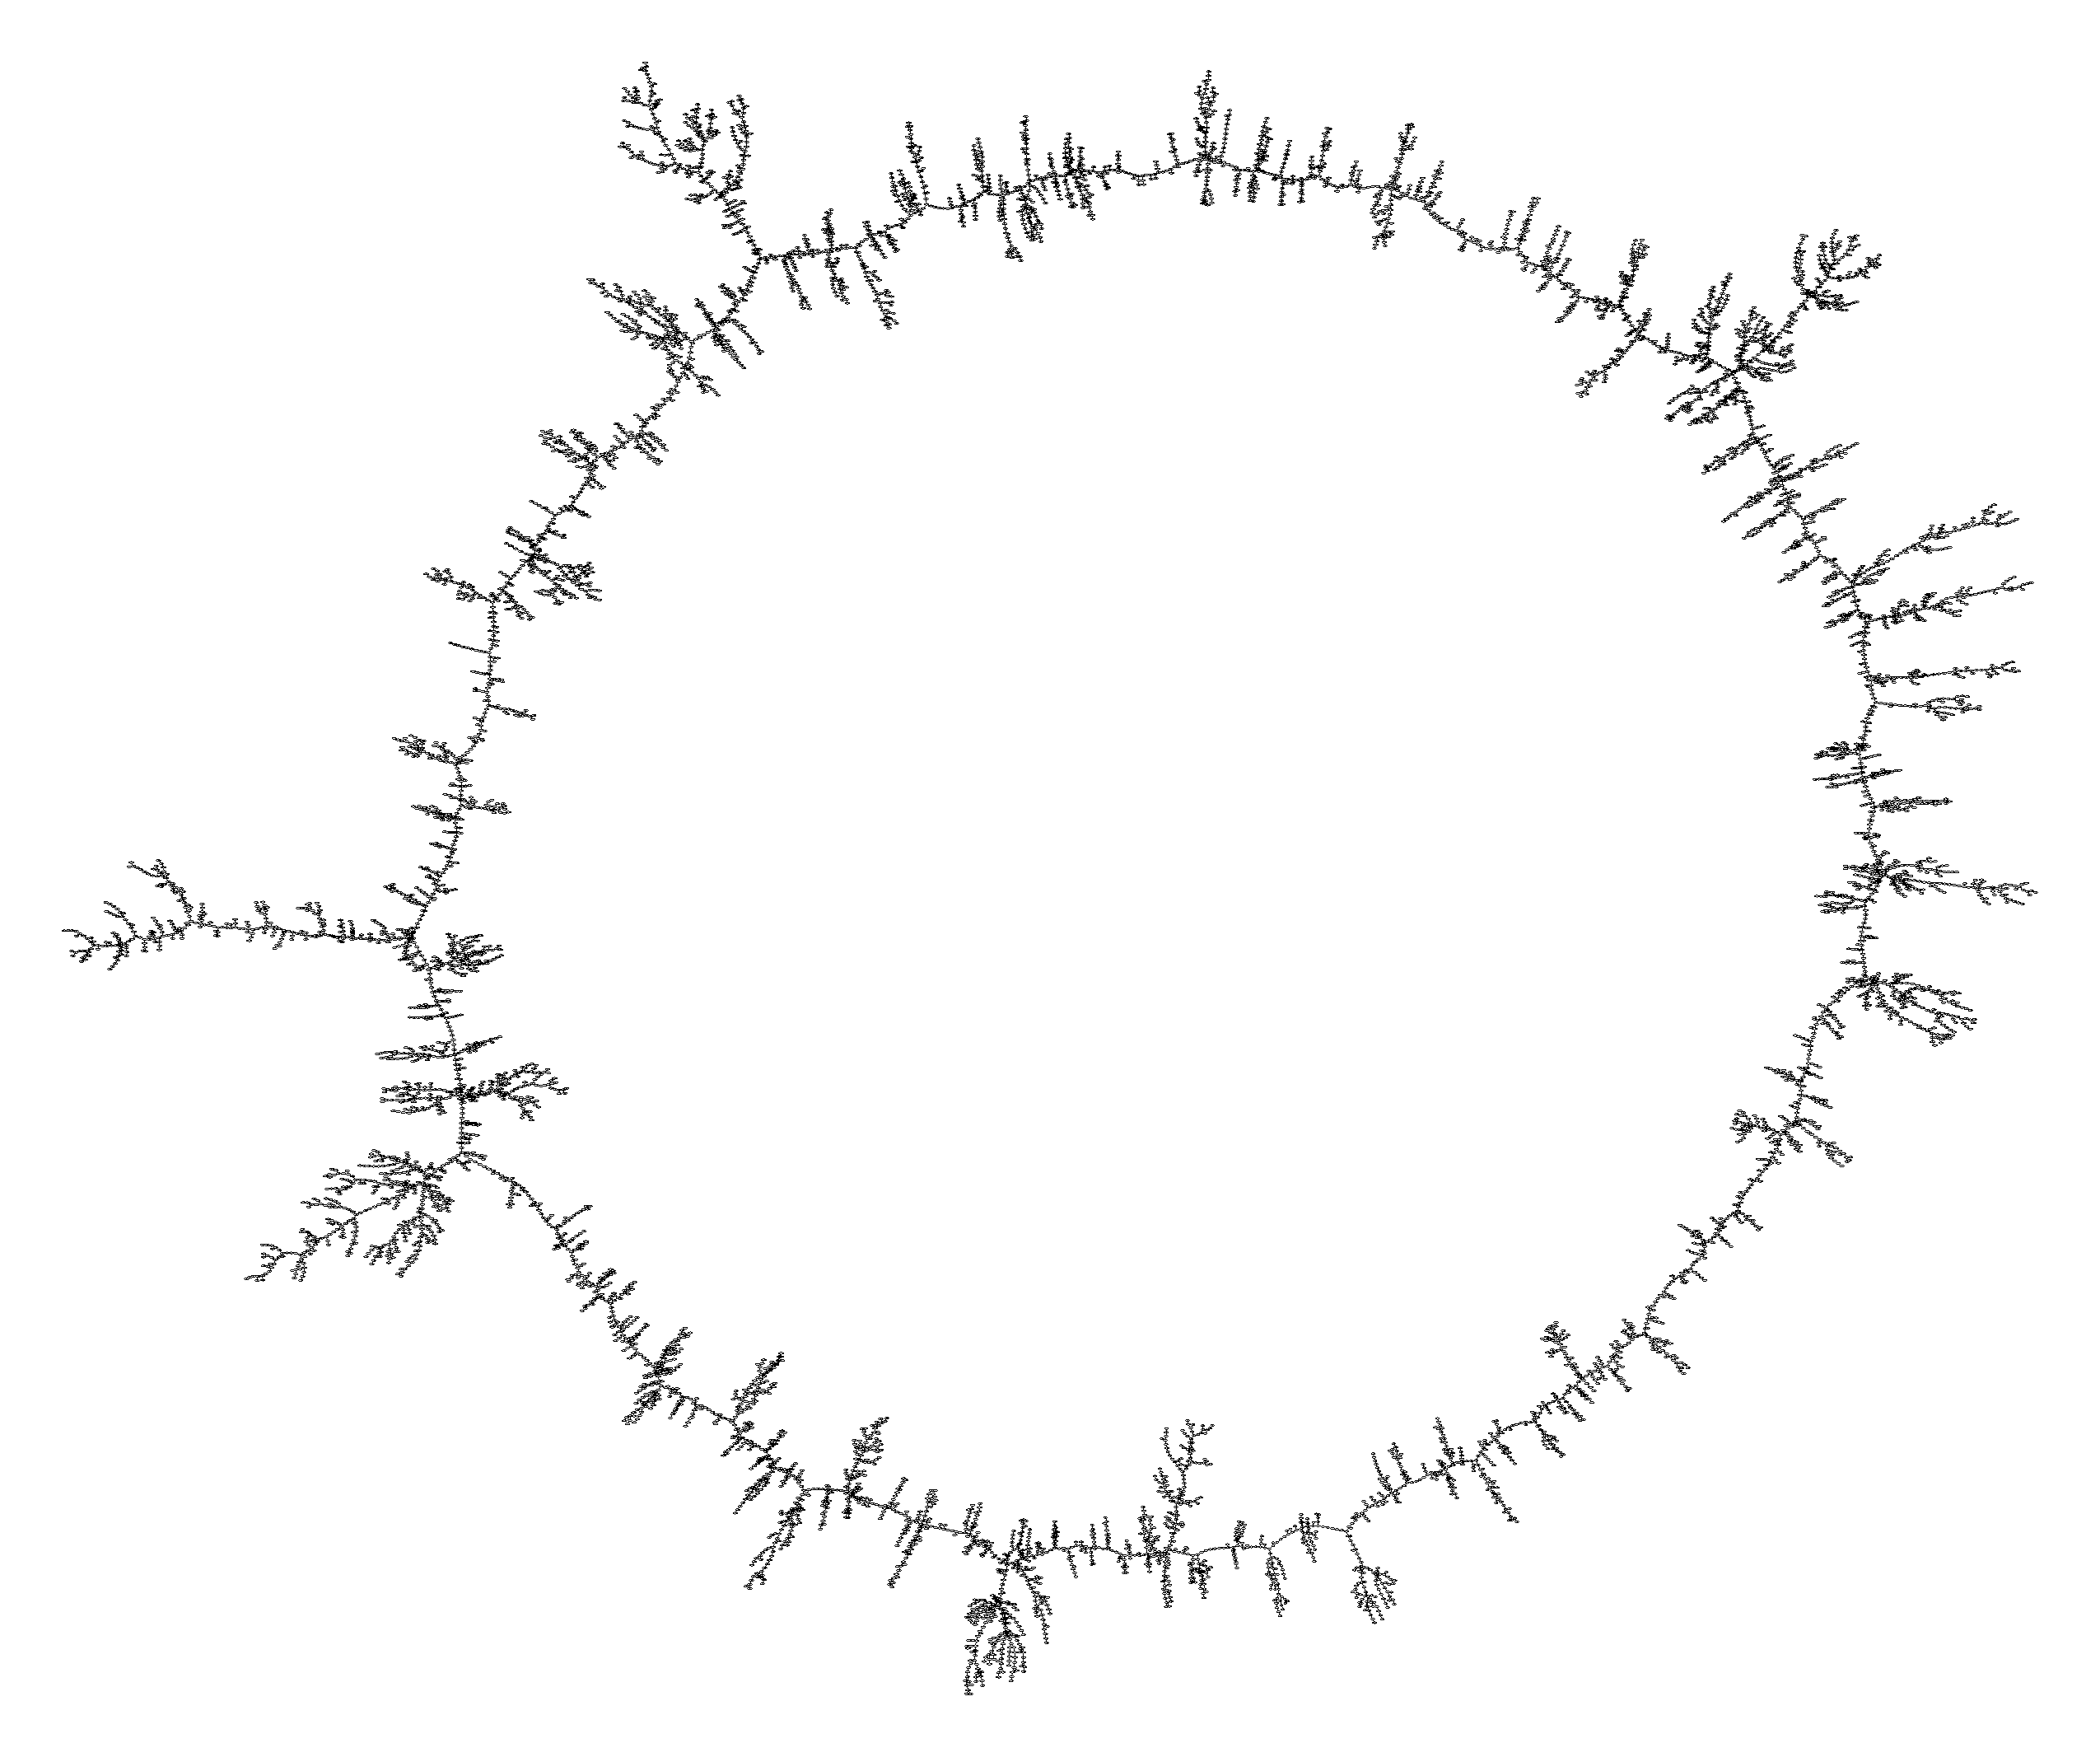
\includegraphics[width=3in]{figures/f3b015}
\caption{Graph visualizations demonstrating the decreasing 
fidelity of graph structure with increasing false positive rate. From 
top left to bottom right, the false positive rates are 0.01, 0.05, 0.10, 
and 0.15.}
\end{figure}

In addition, it is simple to see that a linear increase in the false 
positive rate results in a linear increase in the number of expected 
neighbors for a particular k-mer. For an isolated k-mer (no adjacent 
``real'' k-mers), the calculation is 
E(erroneous neighbors)$ = 8 \times p_f$. This implies that the local graph 
structure breaks down in a linear fashion but offers no insight 
to how the global graph structure degrades.
\marginpar{Whatever happened to the graph/table showing the \# of neighbors with false
positive rate?}
% @JAP if it is the graph you are thinking of, I am not sure that I 
% ever incorporated it into the paper, unless you are thinking of something 
% Arend did. if it is that graph, then I didn't think to include it 
% because the linear effect seems to be intuitive

\subsection{Global Breakdown In K-mer Graphs}
\marginpar{Intro sequence needs strengthening.}
We wanted to explore the point where our data structure becomes unusable, 
so we randomly inserted 31-mers into Bloom
filters with increasing false positive rates and calculated the average
cluster size for each false positive rate. Figure 2 demonstrates that 
the average cluster
size rapidly increases as a specific threshold is approached,
which appears to be at a FP rate near 0.18 for k=31. This
graph also suggests that up to this threshold, DNA assembly graph 
traversal remains feasible but becomes slower as the threshold is
approached.

\begin{figure}
\center{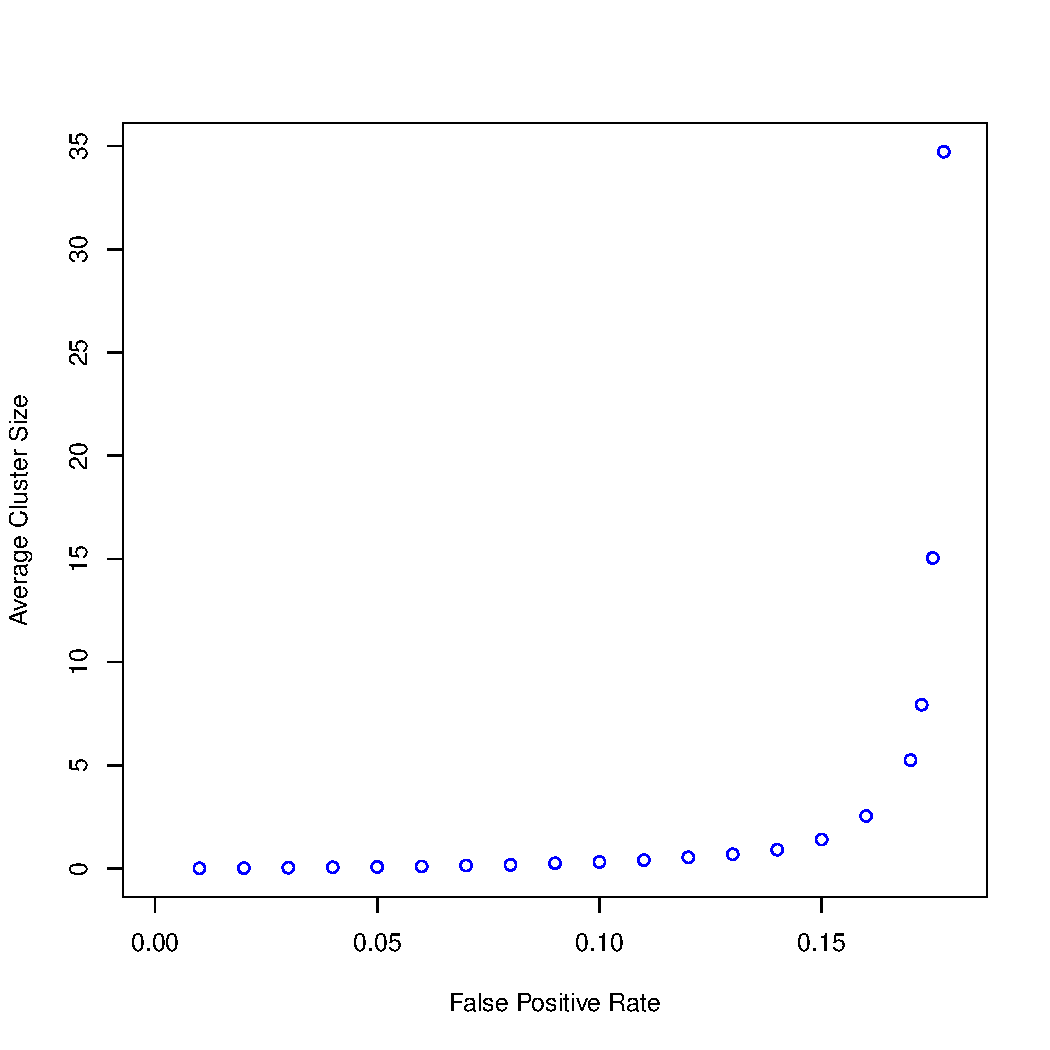
\includegraphics[width=5in]{k31}}
\caption{The average cluster size sharply increases as the false positive 
rate approaches the percolation threshold.
}
\end{figure}

As the false positive rate increases, there appears to be a sudden
transition between the point where graph traversal is feasible and
when it is not (Figure 2). This rapid change appears to resemble 
a phase transition in the
field of physics, which can be modelled using percolation theory. As
\marginpar{This is awfully fast.  Can you expand on this a bit?  Also, my
addition of ``appears to resemble'' is awfully wishy-washy.  Feel free to
change.}
long as the false positive rate is below the percolation threshold (in
the subcritical phase), it is feasible to traverse the graph. If the
false positive rate is at or above this (in the supercritical phase), then graph
traversal is infeasible.
% @JAP I have thought this previously, but I cannot think of a good 
% way to ``ease'' into the topic of percolation theory

Using the calculation method described in \emph{Methods}, we found that the 
site percolation threshold for de Bruijn graphs is $\sim0.183$. 
The percolation threshold appears to be the same for 
different $k$, which suggests that the 
critical point is $k$ independent. This implies that as long as the 
false positive rate is below $\sim 0.183$, connected components in the graph 
are unlikely to erroneously connect to one another.
\marginpar{Evidence for k independence?  And do we want to just say ``fp rate is below 0.18'' or keep the ``approximately'' in there?}

\subsection{Large-scale Graph Structure Retained to Percolation Threshold}
We wanted to know if the global connectivity of the graph is unlikely 
to change below the percolation threhold. 
The diameter of a connected component in a graph is a measure of 
the length of the ``longest shortest'' 
path between any two vertices\cite{bondy2008graph}.
In our case, we only considered paths between two real k-mers
in the dataset for the only component that contains real k-mers. 
We randomly generated 50bp long circular
chromosomes to construct components containing 50 k-mers and 
calculated the diameter at different false positive rates, averaging
the results from multiple runs ($n=20$).
\marginpar{k is 8 here?  and how tough would it be to do n=100?  and aren't
there L-k+1 k-mers in an L-length sequence?}
% I had to set k to be low because I wanted to go beyond the percolation
% threshold, and I couldn't think of a straightforward way to handle it
% for a high value of k...n=100 or whatever would be pretty easy...I just 
% wanted to get the graph generated
As Figure 3 shows, 
erroneous connections between pairs of ``real'' k-mers are unlikely
below the 
percolation threshold. At or after the percolation threshold, spurious connections 
between real k-mers are created, which lowers the diameter. For larger k, false connections 
between k-mers are even more unlikely since the shortest path between two k-mers 
with no overlap is $k$ in length.\marginpar{Is this true?  I would not really expect this graph to change for different k.  Can it be tested quickly/easily?  Also, can we calculate this analytically for a simple situation?}
% @JAP for 3-mers, you would need three k-mers to get from AAA to CCC
% bump that up to 4-mers, and for the same false positive rate 
% you are less likely to connect AAAA to CCCC than AAA to CCC

\begin{figure}
\center{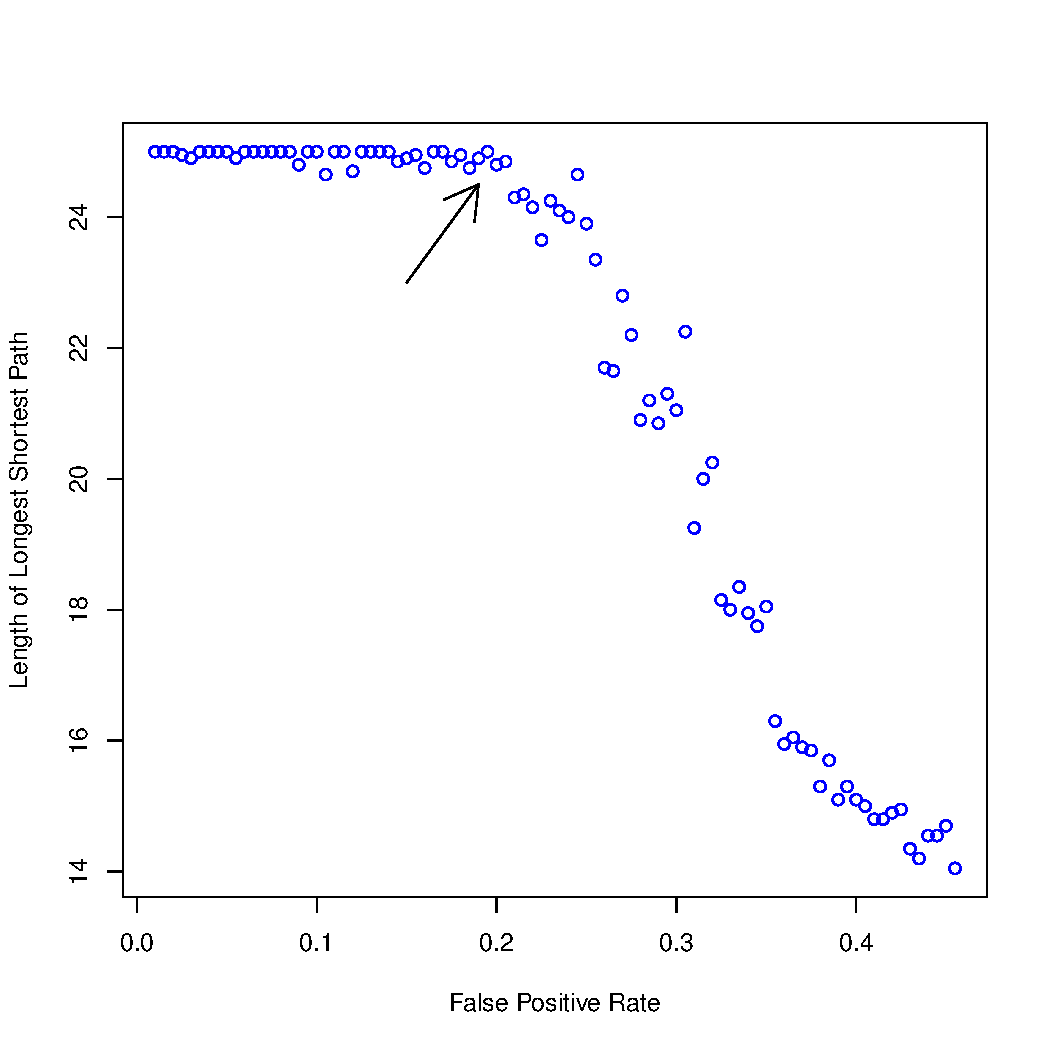
\includegraphics[width=5in]{figures/diameter}}
\caption{The length of the longest shortest path of randomly generated 50bp 
long circular chromosomes in 8-mer 
space for different false positive rates. Only real (non-error) k-mers are
considered for starting and ending points.  @CTB change FPR in figure title to ``false positive rate''; move the title into the caption.}
\end{figure}

\subsection{Sequencing Errors Eclipse Errors From Graph Representation}
One important consideration when determining the usefulness of our k-mer
graph representation is how it compares to errors from massively
parallel sequencers such as Illumina. In de Bruijn graph-based
assemblers, sequencing errors add to the graph complexity and make it
more difficult to find high-quality paths for generating long,
accurate contigs. Since our approach generates
false positives, we aim to show that sequencing errors dominate the graph complexity
issue. We used an E. coli dataset provided by Illumina to compare
various graph invariants between the Illumina dataset, an exact
representation of the genome, and various inexact representations with
different false positive rates.

\begin{figure}
\begin{tabular}{ | c || c | c | c | c | c | }
\hline
 & No. K-mers & No. Additional & No. Missing & Deg $\ge 2$ & \% Real K-mers \\ \hline \hline
\emph{E. coli} Exact & 4530123 & 0 & 0 & 50605 & 100 \\ \hline
\emph{E. coli} 1 \% & 4814050 & 283927 & 0 & 313844 & 94.1 \\ \hline
\emph{E. coli} 5 \% & 6349301 & 1819178 & 0 & 1339102 & 71.3 \\ \hline
Reads Exact & 45566033 & 41036029 & 119 & 7700483 & 9.9 \\ \hline
Reads 1 \% & 48237038 & 43707032 & 117 & 9771028 & 9.4 \\ \hline
Reads 5 \% & 62094757 & 57564749 & 115 & 18116934 & 7.3 \\
\hline
\end{tabular}
\caption{An exact \emph{E. coli} genome representation of 17-mers was compared with 
two inexact ones as well as an exact and two inexact representations of an Illumina 
\emph{E. coli} dataset.}
\end{figure}

For these estimates, we used an \emph{E. coli} genome and an Illumina 
dataset of the same strain for the comparison using a $k$ value of 17. We found 
that there were 50,605 17-mers in the exact representation that had greater than 
2 degrees. As the false positive rate increased, the number of these 
17-mers increased in the expected linear fashion as well as the number of 
additional 17-mers. Furthermore, the number of 
``real'' 17-mers, those that are not false positives, 
comprise of the majority of the graph.

On the other hand, when we compared an exact representation of an Illumina dataset, 
only 9.9 \% of the k-mers in the graph truly exist in the dataset. Note 
that we only counted false positive k-mers that are in the same component as 
at least one real k-mer. Furthermore, the number of 17-mers with more than 
2 neighbors is proportionally higher than for the exact representation of the 
genome, which demonstrates that sequencing errors greatly add to the complexity 
of the graph. Thus, we find that the errors demonstrated by 
sequencers dwarf the errors caused by our inexact graph representation 
below a reasonable false positive rate.

\section{Discussion}

\subsection{Bloom Filters Can Be Used To Accurately Store Large Assembly Graphs}
The compressible graph representation we have built on a Bloom filter
is an efficient way to store and traverse k-mer graphs.  Per k-mer
memory usage is low compared to exact approaches without false positives,
and memory usage is independent of k.  K-mer vertex lookup and
local traversal are constant time.  The primary data structure can
also be implemented in constant memory.  This graph representation is
also easy to implement correctly.
\marginpar{Is local traversal really constant time?  What is local traversal, anyway?  (I'm aware I wrote that in the first place, yes ;)}

The probabilistic nature of the data structure is a significant
concern, but the collision rate and resulting increase in false local
connectivity are predictable.  On a larger scale, we can link the
rate of increase in global connectivity from false positives to a
first-order phase transition, which lets us define a broad range of
parameters for which the global graph structure is extremely accurate.
Within this range, the primary effect of decreasing memory is to increase
traversal computation.  Note that this also provides a systematic way
to trade time spent in traversal (computation) off against memory. As shown 
in Figure 2, the amount of traversal from each k-mer increases 
(affecting computation) as the false positive rate increases, which 
is determined by the amount of memory that is allocated to the data 
structure.

The effect of increasing false positive rate as ``error'' can be
compared to the effect of sequencing errors.  Sequencing error
introduces both false negatives (by eliminating ``true'' k-mers from
low coverage samples) and false positives.  Novel k-mers
from sequencing errors also often result in k-mers that are
a low Hamming distance from the true k-mer, which can result in
elaborate graph structures.  In contrast, the Bloom graph error is
entirely one-sided, only resulting in false positives; moreover, these
false positives are uncorrelated with the ``true'' k-mers from which
they arise, and generally contribute to local graph structure only 
in a linear fashion as the false positive rate increases.
\marginpar{Should we discuss the role that the hash function plays in
``correlation''?}

Overall, the Bloom k-mer graph is an efficient data structure for
storing and traversing large k-mer graphs.

\subsection{Applying Bloom K-mer Graphs To DNA Sequence Assembly}
Bloom k-mer graphs may not be directly useful for traditional
approaches to DNA assembly, which rely on systematic heuristic
transformations of graph structure to find an optimal path through the
graph.  This is because the Bloom graph, as presented here, is limited
to representing k-mer graphs for a fixed k, and paths cannot readily
be compacted or eliminated.
% @CTB What did I mean ``for a fixed k''?  I don't know of any DBG
% reps that don't use a fixed k!

There are many uses, however, for an extremely scalable
graph representation.  Below we discuss the use of the
Bloom k-mer graph data structure as a vehicle for exploring graph
properties and filtering data sets.

For low-coverage samples, assembly graphs may contain many small
unconnected components, that represent unconnected sequences.
% @CTB why?  Beacuse of low coverage! Reiterate I guess.
Sequences contributing to these unconnected components can be safely
eliminated from the originating data sets without affecting the final
assembly.  This can be done efficiently with a simple limited depth
graph search algorithm. Since connected components in the graph 
are unlikely to erroneously connect when the false positive rate 
is below the percolation threshold, graph traversal is only affected 
by the minor changes to the local graph structure.

More generally, assembly graphs may contain many disconnected
subgraphs, due to the structure of the source data (e.g. transcriptome
or metagenome sequencing) or because of low coverage.  These subgraphs
can safely be partitioned into separate graphs without affecting the
final assembly, reducing the memory and computation required for
assembly of the whole to that required for the largest subgraph.
% @CTB discuss local vs global structure changes from FP on this.
\marginpar{Do we have any references for this anywhere?  Maybe
meta-idb/metavelvet, or the Trinity paper?}

The Bloom k-mer graph can also be used to do de novo repeat discovery
in collections of unassembled reads.  This in turn can be applied to
filtering of repeats prior to assembly/cite{hydra}, or for isolating
repeats from shallow or exploratory sequencing efforts.

It may also be possible to adapt sequence structure (e.g. ORF),
homology (BLAST), and domain search (HMMER) algorithms to search this
graph structure instead of searching either unassembled reads or
assemblies (Fish, Brown and Cole, pers communication).  Because 
assembly graphs implicitly collapse identical
sequences into a single path, this may be a more scalable approach to
targetted-gene analysis for metagenomics than current approaches
(which rely on searching individual reads that may be overlapping or identical).  Also note that, unlike
sequencing errors, the false positives in the Bloom graph will
generally bear no resemblance to biologically valid matches, which 
makes their detection during graph traversal easier.

The Bloom k-mer graph could also be used to develop connectivity-based
read trimming and correction algorithms.  For example, low-abundance
reads that contribute to ``spurs'' or ``sidings'' in otherwise
high-coverage regions could be corrected to match the
consensus, or trimmed to eliminate the divergent sequence.

One particularly intriguing option is to use the memory-efficient and
scalable Bloom k-mer graph representation as a component of a hybrid
assembler.  The k-mer graph approach could be used to identify
reads that belong to high-complexity regions, and extract them for
later resolution with more targetted approaches, e.g. an OLC assembler.
Alternatively, regions could be locally examined and extracted for
assembly, and then passed to scaffolding toolkit like Bambus for 
larger-scale connectivity\cite{bambus}.

\subsection{Dramatic Scaling}
It is clear that sequencing capacity will continue to outpace Moore's 
law and new methods must address this. Our graph representation allows 
for excellent scaling capabilities at the cost of a manageable false positive rate. 
As mentioned previously, $\sim 6.22$ bits per k-mer are required for a 
false positve rate of 5\%, so that modern computers with 
over 512GB of memory can handle graphs containing hundreds of billions of k-mers.

Another consideration is that assembly is generally difficult to parallelize. 
ABySS and Contrail (citation?), for example, place different parts of the 
graph on separate nodes. However, this can hinder performance due to 
network latency. Having the ability to examine the entire graph in memory 
before distributing the graph across multiple processors can minimize the
degree to which processors need to query one another. A smaller memory 
footprint can also mean that the entire assembly could be performed on 
a single node, if computational resources are limited.\marginpar{...if we
build an assembler on this sucker, no?}

Finally, though so-called ``third-generation'' sequencers are showing promise with 
longer reads and better error rates, we believe that improvements in these 
areas will not solve the scaling issue in certain domains. In particular, 
mRNAseq and metagenomics datasets are still sensitive to sampling depth as
well as read length. Differential expression detection and assembly 
of low-expressed genes are difficult without deep coverage. Thus
the required coverage level for an mRNAseq dataset is high, leading to large
data sets. Furthermore, many environmental samples with 
diverse microbial communities are estimated to require several terabases of sequencing 
in order to achieve a modest coverage level (citation?  my refs CTB). In both of these domains, better 
scaling algorithms are needed to handle these complex assemblies. 

\subsection{Concluding Remarks}
We have shown that representing a k-mer graph on a Bloom filter-like data 
structure can create an inexact, yet lightweight graph representation of 
a k-mer graph. This inexactness can be precisely known based on the occupancy 
of each hash table, and we demonstrated that our approach is still useful 
below a specific false positive rate. We conclude that while this representation 
may not be ideal for a final assembly, it can be useful for pre-filtering 
strategies and solving the scaling and memory bottleneck problems that we 
currently face in sequence assembly.

\subsection{Acknowledgements}

Jim Cole and Jordan Fish.  Qingpeng.  Adina.  Adami.  JGI folk.

\bibliographystyle{abbrv}
\bibliography{kmer-percolation}
\end{document}


